\section{Identifying Metamorphic Transformations} \label{identifyingMR}
Some common problems with images are that they can have some small random rotations, or they could be located a bit off from the center, or the exposure of the picture could be high. These problems with images prompted us to look into affine transformations as a possible set of transformations to use for this project. To answer our first research question, we implemented some affine transformations on the datasets as possible candidates for metamorphic properties. We observed that applying these affine transformations on the dataset to a very small degree produced similar accuracy as that of the original dataset. Thus we selected these five transformations as metamorphic properties for each dataset: rotate, shear, shade, shift the image along $x$-axis, and shift the image along $y$-axis. It should be noted that there more affine transformations than the five we identified, and they can be used as metamorphic transformation as well. However, these transformations appear to be the most common ways one can manipulate image datasets. Each image in the testing dataset (MNIST, Fashion-MNIST, and EMNIST-Letter) was transformed using these five metamorphic properties. We used Keras image preprocessing functions to apply these transformations to the test data in each dataset to generate new data to measure robustness.

After some primary investigation using the transformed datasets and some standard machine learning algorithms, we saw that the machine learning algorithms produced very similar accuracies on datasets, which were very similar to the original dataset. Thus, we defined our metamorphic relation as "a small change in the input from a known test case should lead to a similarly small change (or no change) in the output." We use this metamorphic relation for all the transformations.

There are $10000$ test images in the MNIST dataset. There are $10$ class labels from $0$ to $9$, and each class label has $1000$ samples. We applied the following metamorphic properties to each test image.
\subsection{Rotate}
% Since we are dealing with image datasets, we hypothesize that small changes to the images by rotating them clock-wise or counter clock wise would not have drastic effect on the accuracy of model. To test our hypothesis we rotated the test data at each angle between [\ang{-50}, \ang{50}]. 
The first metamorphic property we identified was rotating the images on the $z$ axis. To implement the rotate property, we used the Keras ImageDataGenerator class. ImageDataGenerator implements $apply\_transform()$ method, which can be used to rotate images by passing the argument $'theta'$ along with the angle to rotate the image. Every image in the three datasets was rotated for every angle in [$-50$, $50$]. This generated 100 versions of the follow-up test dataset of the original data, where each version differs from the last by $1$ degree of rotation. We expect that certain digits with symmetry (like $0$) will not be affected that much by the rotate property. 
% The test images from each dataset is transformed For each angle in [\ang{-50}, \ang{50}] we transformed each image Each image (digit, letter, and, fashion) is rotated clockwise and counter clockwise between angles [\ang{-50}, \ang{50}].  The rotation transformation algorithm takes in an image and an angle in degrees as parameter and rotates the image with the given angle. 
    \begin{figure}[!htbp]
        \centering
        \begin{subfigure}[b]{.3\textwidth}
            \centering
            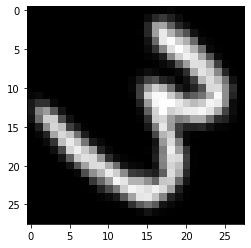
\includegraphics[width=\linewidth]{images/rotate1.png}
            \caption{Angle: \ang{-50}}
            \label{fig:Rotate-misclass0}
        \end{subfigure}%
        \begin{subfigure}[b]{.3\textwidth}
            \centering
            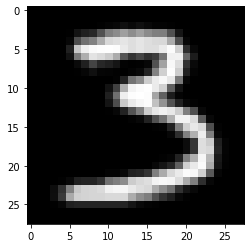
\includegraphics[width=\textwidth]{images/rotate2.png}
            \caption{Angle: \ang{0}}
            \label{fig:Rotate-misclass0}
        \end{subfigure}%
        \begin{subfigure}[b]{.3\textwidth}
            \centering
            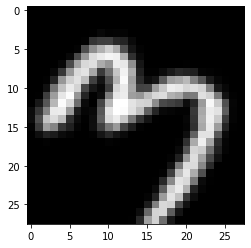
\includegraphics[width=\linewidth]{images/rotate3.png}
            \caption{Angle: \ang{50}}
            \label{fig:Rotate-misclass0}
        \end{subfigure}
        \caption{Rotate property applied to Digit 3.}
        \label{fig:Rotate-property}
    \end{figure}
    \FloatBarrier
    
\subsection{Shade}
We represent the pixels of the MNIST images as floating point numbers between 0 and 1 where 0 is white, and 1 represents black. To apply the shade transformation, we increased the non-black pixels by $0.01$ for every image until they became black.
    \begin{figure}[htb!]
        \centering
        \begin{subfigure}[b]{.3\textwidth}
            \centering
            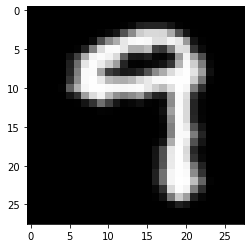
\includegraphics[width=\linewidth]{images/shade1.png}
            \caption{Shading Value: 0}
            \label{fig:Rotate-misclass0}
        \end{subfigure}%
        \begin{subfigure}[b]{.3\textwidth}
            \centering
            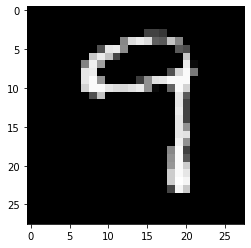
\includegraphics[width=\textwidth]{images/shade2.png}
            \caption{Shading Value: 0.80}
            \label{fig:Rotate-misclass0}
        \end{subfigure}%
        \begin{subfigure}[b]{.3\textwidth}
            \centering
            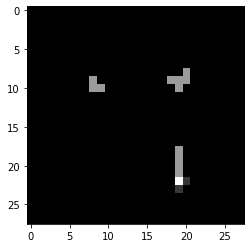
\includegraphics[width=\linewidth]{images/shade3.png}
            \caption{Shading Value: 0. 99}
            \label{fig:Rotate-misclass0}
        \end{subfigure}
        
        \caption{Shade property applied to Digit 9.}
        \label{fig:Shade-property}
    \end{figure}
    \FloatBarrier
    
\subsection{Shear} 
To shear the images, we used the image pre-processing library offered by Keras. The ImageDataGenerator class generates batches of tensor image data with real-time data augmentation. We used the ImageDataGenerator's $apply\_transform()$ method to apply a transformation to an image according to given parameters. The $apply\_transform()$ method takes in the image, transformation type, and, the amount of transformation to be applied as a parameter. It then applies the transformation and returns a transformed version of the input in the same shape.
The transformation parameter we used here was $shear$, and the images were transformed for every angle in $[-50, 50]$.

    \begin{figure}[!htbp]
        \centering
        \begin{subfigure}[b]{.3\textwidth}
            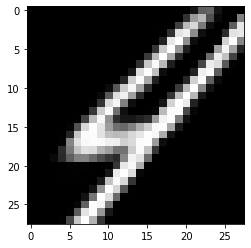
\includegraphics[width=\linewidth]{images/shear1.png}
            \caption{Angle: \ang{-50}}
            \label{fig:Rotate-misclass0}
        \end{subfigure}%
        \begin{subfigure}[b]{.3\textwidth}
            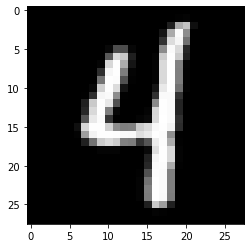
\includegraphics[width=\textwidth]{images/shear2.png}
            \caption{Angle: \ang{-50}}
            \label{fig:Rotate-misclass0}
        \end{subfigure}%
        \begin{subfigure}[b]{.3\textwidth}
            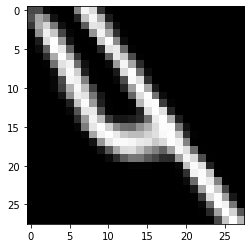
\includegraphics[width=\linewidth]{images/shear3.png}
            \caption{Angle: \ang{-50}}
            \label{fig:Rotate-misclass0}
        \end{subfigure}
        
        \caption{Shear property applied to Digit 4.}
        \label{fig:Shear-property}
    \end{figure}
    \FloatBarrier
    
\subsection{Shift the image along the X axis(ShiftX)}
Since the images are $28$ pixels wide, shifting the images by more than 28 pixels in either direction moved the images out of the frame completely. Thus, we transformed the test datasets by moving each image by pixels between 0 and 28 in both the X directions. We used ImageDataGenerator's $apply\_transform()$ function with $tx$ parameter and a pixel value in order to perform this transformation. This generated 56 follow-up test dataset of the original data where each version differs from the last by $1$ pixel shift along the $x$ axis.
    \begin{figure}[htb!]
        \centering
        \begin{subfigure}[b]{.3\textwidth}
            \centering
            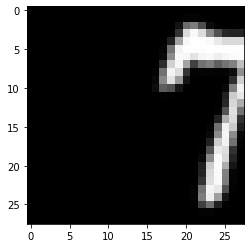
\includegraphics[width=\linewidth]{images/shiftx1.png}
            \caption{Pixel shift: 10}
            \label{fig:Rotate-misclass0}
        \end{subfigure}%
        \begin{subfigure}[b]{.3\textwidth}
            \centering
            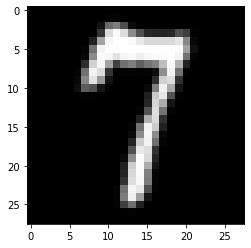
\includegraphics[width=\textwidth]{images/shiftx2.png}
            \caption{Pixel shift: 0}
            \label{fig:Rotate-misclass0}
        \end{subfigure}%
        \begin{subfigure}[b]{.3\textwidth}
            \centering
            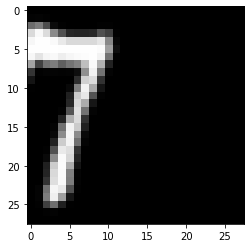
\includegraphics[width=\linewidth]{images/shiftx3.png}
            \caption{Pixel shift: -10}
            \label{fig:Rotate-misclass0}
        \end{subfigure}
        
        \caption{ShiftX property applied to Digit 7.}
        \label{fig:ShiftX-property}
    \end{figure}
    \FloatBarrier
    
\subsection{Shift the image along the Y axis(ShiftY)}
The last metamorphic property we identified was shifting the images on the Y-axis. We used ImageDataGenerator's $apply\_transform()$ function with $ty$ parameter to transform the test data. Since the images are 28x28 pixels, we shifted the images by each pixel between 0 and 28 pixels in both Y directions. 
    \begin{figure}[htb!]
        \centering
        \begin{subfigure}[b]{.3\textwidth}
            \centering
            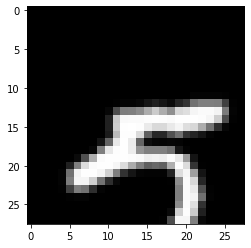
\includegraphics[width=\linewidth]{images/shifty1.png}
            \caption{Pixel shift: -10}
            \label{fig:Rotate-misclass0}
        \end{subfigure}%
        \begin{subfigure}[b]{.3\textwidth}
            \centering
            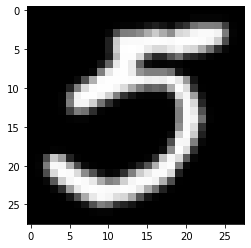
\includegraphics[width=\textwidth]{images/shifty2.png}
            \caption{Pixel shift: 0}
            \label{fig:Rotate-misclass0}
        \end{subfigure}%
        \begin{subfigure}[b]{.3\textwidth}
            \centering
            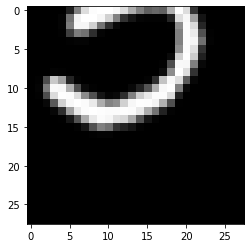
\includegraphics[width=\linewidth]{images/shifty3.png}
            \caption{Pixel shift: 10}
            \label{fig:Rotate-misclass0}
        \end{subfigure}
        
        \caption{ShiftY property applied to Digit 5.}
        \label{fig:ShiftY-property}
    \end{figure}
    \FloatBarrier

The follow-up test images have the same structure and labels as the original image. After generating all the transformed versions of the datasets, they were saved to be used as follow-up test cases for our machine-learning algorithms. The section \ref{identifyingMR} also answers our first research question.
